\documentclass[t]{beamer}
\setbeameroption{show notes}
%hide all notes
%\setbeameroption{hide notes}

% German style date formatting (footer)
\usepackage[ddmmyyyy]{datetime}
\renewcommand{\dateseparator}{.}

% Format the captions used for figures etc.
\usepackage[compatibility=false]{caption}
\captionsetup{singlelinecheck=off,justification=raggedleft,labelformat=empty,labelsep=none}



\usepackage{etex} % cures ``No room for a new \dimen'' error

%%%%%% font size handling %%%%%%
\RequirePackage{fix-cm}
\usepackage{lmodern}
\DeclareFontFamily{OMX}{lmex}{} % proper math mode size (http://tex.stackexchange.com/questions/74623/big-integral-in-lmodern)
\DeclareFontShape{OMX}{lmex}{m}{n}{<-> lmex10}{}
% \addtokomafont{disposition}{\rmfamily}

%%%%%% better enumerate environment
\usepackage{enumitem}

%%%%%% bold math %%%%% (boldsymbol)
\usepackage{bm}

%%%%%% textdegree %%%%%
\usepackage{ textcomp }

%%%%%% tikz %%%%%%
% \usepackage{pdfpages}
\usepackage{pgfplots}
\pgfplotsset{compat=newest}
\usepackage{tikz}
\usetikzlibrary{fit}

\usetikzlibrary{arrows}
\usetikzlibrary{arrows.meta} % propper scaling of arrows
\pgfplotsset{plot coordinates/math parser=false}
\usetikzlibrary{plotmarks}
% \usetikzlibrary{decorations.shapes}
% \usetikzlibrary{decorations.pathmorphing}
\usepgfplotslibrary{fillbetween}
\usetikzlibrary{patterns}
\usetikzlibrary{intersections}
% \usetikzlibrary{decorations.markings}
% \usetikzlibrary{arrows.meta}
\usepackage{graphicx}
\usepackage{amssymb}
\usepackage{multimedia}
\usepackage{array}
\usepackage{booktabs,adjustbox}
\usepackage{marvosym}
\usepackage{hyperref}
\usetikzlibrary{calc}
% \usepackage{animate}
% \usepackage{movie15}
\usepackage{pdfpages}
\usepackage{pifont}
\newcommand{\cmark}{\ding{51}}%
\usepackage[thinlines]{easytable}

%%%%%% additional packages %%%%%%
% \usepackage{wrapfig}
\usepackage[absolute,overlay]{textpos}
\usetikzlibrary{positioning}
\usepackage{arydshln}
\usepackage{setspace}
\usepackage{multirow}
\usepackage{multicol}
\usepackage{import}
\usepackage{mathtools}

\usepackage{diagbox}
\usetikzlibrary{matrix}


%%%%%% plot sizes %%%%%%
\def\plottitlefontsize{\Large}
\def\plotlabelfontsize{\normalsize}
\def\plotlegendfontsize{\scriptsize}
\def\plottickfontsize{\normalsize}
% \def\plottickfontsize{\tiny}
\def\plotlinewidth{1pt}
\def\plotnodefontsize{\small}

\newlength\figureheight
\newlength\figurewidth

%%%%%% triangles as item markers %%%%%%
\setlist[itemize,1]{label={\small\raise2.5pt\hbox{\donotcoloroutermaths{\color{rwth-75}$\blacktriangleright$}}}}
\setlist[itemize,2]{label={\small\raise2.5pt\hbox{\donotcoloroutermaths{\color{rwth}$\triangleright$}}}}




 \usepackage{pdfpages}
%%%%%% a footnote box for references %%%%%%
\newcounter{grcitenumber}
\newcommand{\declcite}[1]{\refstepcounter{grcitenumber}\label{#1}}
% \newcommand{\showcite}[1]{\ensuremath{\grm{^{\mathit{[\ref{#1}]}}}}}
\newcommand{\showcite}[1]{\ensuremath{\grm{^{\mathit{[#1]}}}}}
% % \newcommand{\greycite}{\stepcounter{grcitenumber}{\ensuremath{\bm{^{\mathit{[\thegrcitenumber]}}}}}}
\newcommand{\citetext}[2]{\grm{$\mathit{[#1]:}$\ \textit{#2}}}
\newcommand{\showlargecite}[1]{\grm{$\mathit{[#1]}$}}
\newcommand{\citebox}[2]{\begin{textblock*}{\textwidth}(0.8cm,16.2cm)\setstretch{0.5}\citetext{#1}{#2}\end{textblock*}}
\newcommand{\citeboxx}[4]{\begin{textblock*}{\textwidth}(0.8cm,15.7cm)\setstretch{0.5}\citetext{#1}{#2} \\ \citetext{#3}{#4}  \end{textblock*}}
\newcommand{\citeboxxx}[6]{\begin{textblock*}{\textwidth}(0.8cm,15.2cm)\setstretch{0.5}\citetext{#1}{#2} \\ \citetext{#3}{#4} \\ \citetext{#5}{#6} \end{textblock*}}
\newcommand{\citeboxxxx}[8]{\begin{textblock*}{\textwidth}(0.8cm,14.7cm)\setstretch{0.5}\citetext{#1}{#2} \\ \citetext{#3}{#4} \\ \citetext{#5}{#6} \\ \citetext{#7}{#8} \end{textblock*}}

\def\grm#1{\color{black-75}{#1}\color{black}}
%%%%% theorems %%%%%%
\newtheorem{remark}[theorem]{Remark}

%%%%%% backup slides not counting to page numbers %%%%%%
\newcommand{\backupbegin}{
   \newcounter{finalframe}
   \setcounter{finalframe}{\value{framenumber}}
}
\newcommand{\backupend}{
   \setcounter{framenumber}{\value{finalframe}}
}

%%%%% custom commands %%%%%%
\def\rhf#1{#1 \rfloor} 
\def\prhf#1#2{#1 \rfloor_{#2}} 
\def\lhf#1{\lceil #1}
\def\plhf#1#2{\lceil^{#2} #1}
\def\mean#1{\langle #1 \rangle}
\def\ns#1{\underline{#1}}
\def\ssum#1{\sum_{\substack{#1}}}
\def\sprod#1{\prod_{\substack{#1}}}
\def\ltimes{\times \ldots \times}
\def\lotimes{\otimes \ldots \otimes}
\def\tr#1{{#1}^T}
\def\sp#1#2{\langle #1,#2 \rangle}
\def\sm#1{\mbox{\large\boldmath$($} #1 \mbox{\large\boldmath$)$}}
\def\mean#1{\langle #1 \rangle}
\def\q#1{``#1``}
\def\lhb#1{\mathcal{L}(#1)} 
\def\rhb#1{\mathcal{R}(#1)}

\newcommand{\diver}{\mathop{\rm div}}
\newcommand{\Ind}{\mathcal{I}}
\newcommand{\Index}{\mathcal{I}}
\newcommand{\K}{\ensuremath{\mathbb{K}}}
\newcommand{\R}{\ensuremath{\mathbb{R}}}
\newcommand{\C}{\ensuremath{\mathbb{C}}}
\newcommand{\N}{\ensuremath{\mathbb{N}}}
\newcommand{\Z}{\ensuremath{\mathbb{Z}}}
% \newcommand{\argmin}{\mathop{\rm argmin}}
\DeclareMathOperator*{\argmin}{argmin}
\newcommand*\intd{\mathop{}\!\mathrm{d}}







\usetheme{rwth}

% Setup presentation information
\title{Training DNNs in Tiny Subspaces}
\subtitle{Introductory Talk $|$ Janik Philipps}
\date[RWTH]{Introductory Talk \enskip|\enskip\today}
\author[Max]{Janik Philipps}
\institute[RWTH]{RWTH Aachen}

\logo{
\includegraphics{logo}}

\include{stmaryrd}

\begin{document}

\renewcommand{\C}{\mathbb{C}}								% abbreviation
\newcommand{\E}{\mathbb{E}}									% abbreviation
\renewcommand{\H}{\mathbb{H}}								% abbreviation
\renewcommand{\N}{\mathbb{N}}								% abbreviation
\newcommand{\M}{\mathbb{M}}								% abbreviation
\renewcommand{\R}{\mathbb{R}}								% abbreviation
\renewcommand{\S}{\mathbb{S}}								% abbreviation
\newcommand{\V}{\mathbb{V}}									% abbreviation
\renewcommand{\Z}{\mathbb{Z}}								% abbreviation

\definecolor{def_color}		{RGB}{0,84,159}
\definecolor{def_shade_color}	{RGB}{199,221,242}
\definecolor{def_title_color}	{RGB}{0,84,159}
\definecolor{def_frame_color}	{RGB}{64,127,183}

\definecolor{thm_shade_color}	{RGB}{254,234,201}	
\definecolor{thm_title_color}	{RGB}{0,0,0}
\definecolor{thm_frame_color}	{RGB}{250,190,80}

\setbeamercolor{title page bar}{fg=white}
\setbeamertemplate{title page}[rwth][title_small]{}


\setbeamercolor{block title}{bg=def_frame_color, fg=white}
\setbeamercolor{block body}{bg=def_shade_color, fg=black}
\setbeamercolor{block title alerted}{bg=thm_frame_color, fg=white}
\setbeamercolor{block body alerted}{bg=thm_shade_color, fg=black}



%%%%%%%%%%%%%%%%%%%%%%%%%%%%%%%%%%%%%%%%%%%%%%%%%%%%%%%%%%%%%%%

\begin{frame}[plain]
\titlepage
\end{frame}

%%%%%%%%%%%%%%%%%%%%%%%%%%%%%%%%%%%%%%%%%%%%%%%%%%%%%%%%%%%%%%%

\section{Paper}
\begin{frame}
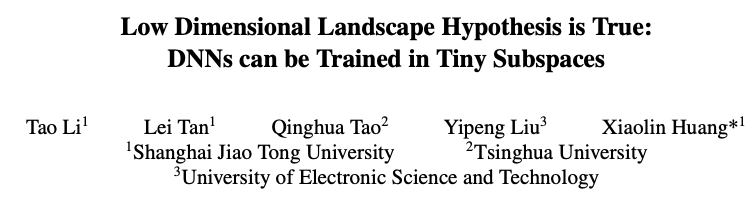
\includegraphics[width=0.99\textwidth]{paper}
\end{frame}



\section{Motivation: Deep neural networks depend on million of parameters causing severe problems}
\begin{frame}
\begin{columns}[c]

\begin{column}{0.5\textwidth}
\begin{center}
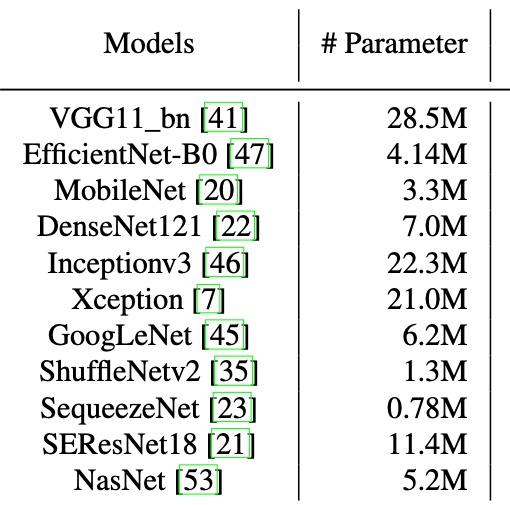
\includegraphics[width=0.99\textwidth]{parameters.png}
\end{center}
\end{column}

\begin{column}{0.5\textwidth}
\begin{itemize}
\item Potential overfitting of the data \vspace{1cm}
\item Only first order methods applicable \vspace{1cm}
\item Computationally and time intensive training \vspace{1cm} 
\item Many training data needed \vspace{1cm}
\item Questionable solution quality  
\end{itemize}
\end{column}

\end{columns}
\end{frame}



\section{Motivation: The number of independent optimization variables may be smaller than the number of parameters}
\begin{frame}
\begin{itemize}
\item Due to strong mutual relationships, \textbf{regarding each parameter} of deep neural networks \textbf{as an independent variable is too rough} \vspace{1cm}
\item The \textbf{gradients of parameters are strongly related} due to the training via backpropagation \vspace{1cm}
\item The parameters in the same layers also have \textbf{synergy correlations} \vspace{1cm}
\end{itemize}
\center{$\downarrow$}\vspace{1cm}
\center{ \fbox{''DNNs can be trained in low-dimensional subspaces''}} \vspace{1cm}
\end{frame}



\section{Motivation: Pioneering work achieved 90\% accuracy in smaller spaces}
\begin{frame}
\begin{itemize}
\item There exists pioneering work on \textbf{training via random projections} \vspace{1cm}
\item For example, on CIFAR-10, LeNet with 62006 parameters could be optimized in 2900-dimensional subspaces with 
\textbf{90\% accuracy of regular SGD training}. \vspace{1cm}
\center{$\downarrow$} \vspace{1cm}
\center{Very promising but we can do even better!} \vspace{1cm}
\item{Many standard neural network architectures could be \textbf{well trained by only 40 independent variables} with almost the same performance. }
\end{itemize}
\end{frame}



\section{Approach in the paper}
\begin{frame}
\begin{columns}[c]

\begin{column}{0.5\textwidth}
\begin{center}
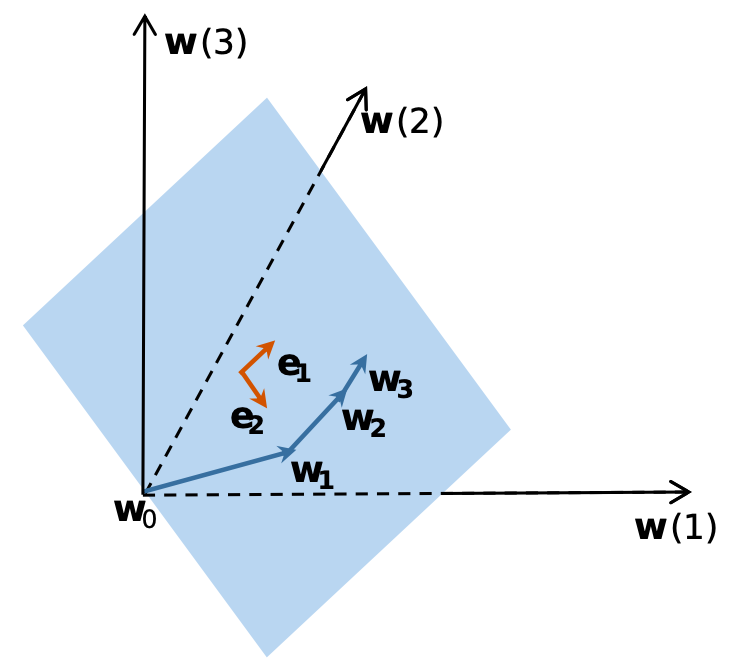
\includegraphics[width=0.99\textwidth]{approach.png}
\end{center}
\end{column}

\begin{column}{0.5\textwidth}
\begin{itemize}
\item There are \textbf{three parameters} $w(1)$, $w(2)$, $w(3)$ \textbf{to optimize}. \vspace{1cm}
\item The training trajectory $\{w_i\}_{i=0,\dots,t}$ could be in a \textbf{two-dimensional subspace} spanned by $e_1$ and $e_2$ \vspace{1cm} 
\item Training in the low-dimensional space can have \textbf{comparable performance} as training in the regular space
\end{itemize}
\end{column}

\end{columns}
\end{frame}



\section{Agenda}
\begin{frame}
\begin{columns}[c]

\begin{column}{0.5\textwidth}
\begin{center}
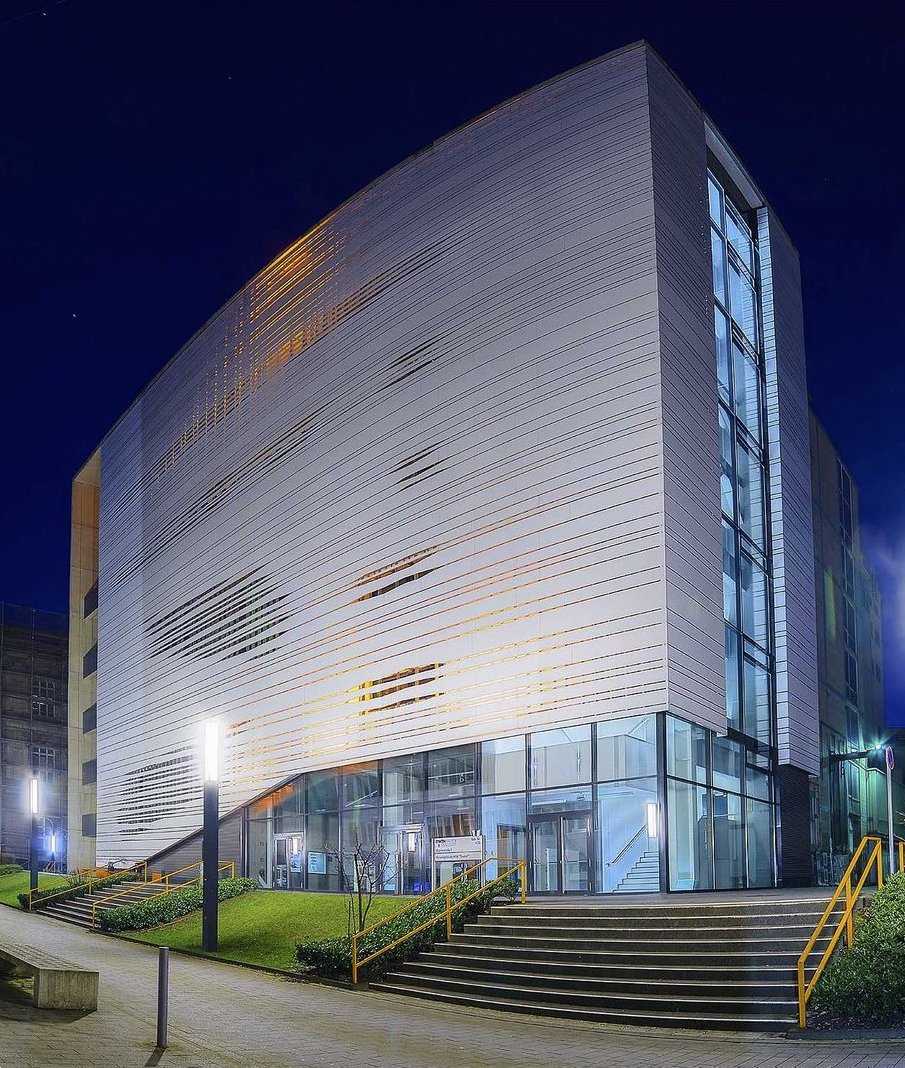
\includegraphics[width=0.9\textwidth]{toaster}
\end{center}
\end{column}

\begin{column}{0.5\textwidth}
\begin{itemize}
\item Dynamic Linear Dimensionality Reduction (DLDR) \vspace{1cm}
\item DLDR-based Quasi-Newton Algorithm \vspace{1cm}
\item Numerical Experiments \vspace{1cm} 
\end{itemize}
\end{column}

\end{columns}
\end{frame}



\begin{frame}

\begin{columns}[c]

\begin{column}{0.5\textwidth}
\begin{center}
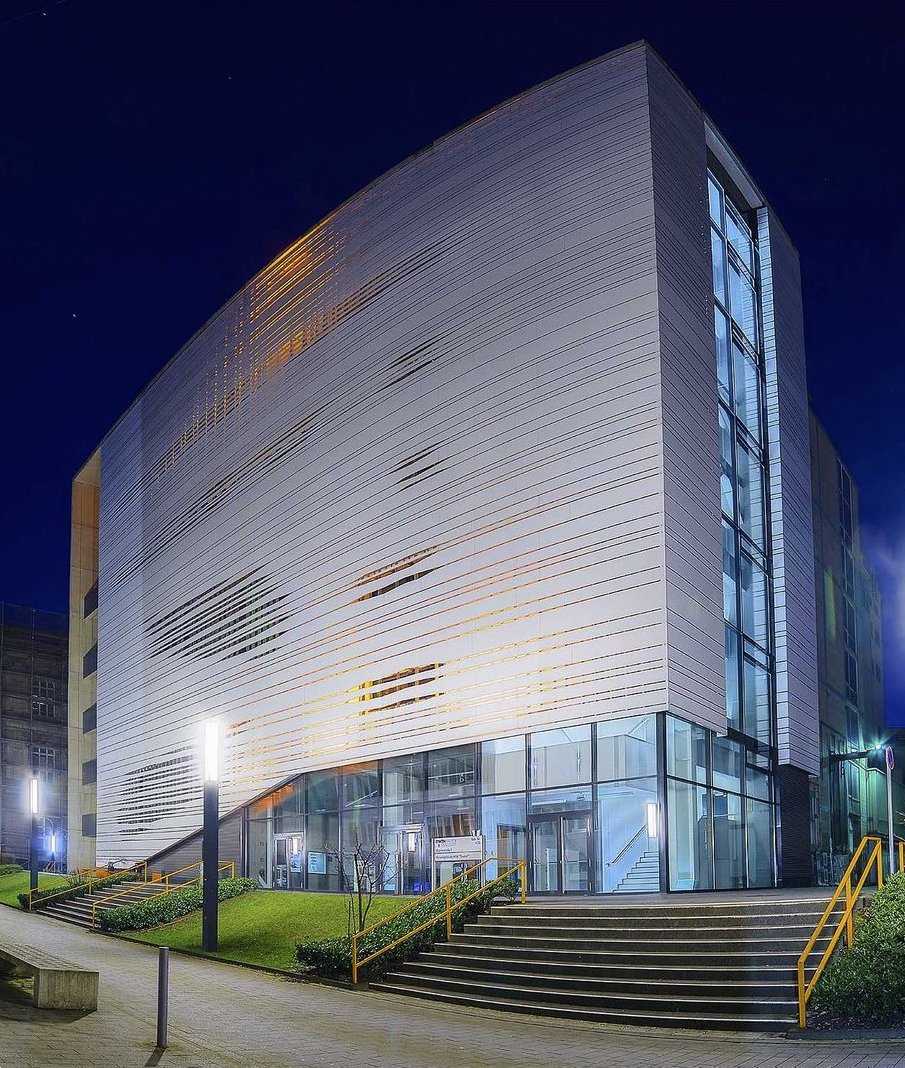
\includegraphics[width=0.9\textwidth]{toaster}
\end{center}
\end{column}

\begin{column}{0.5\textwidth}
\begin{itemize}
\item \textbf{Dynamic Linear Dimensionality Reduction (DLDR)} \vspace{1cm}
\item DLDR-based Quasi-Newton Algorithm \vspace{1cm}
\item Numerical Experiments \vspace{1cm} 
\end{itemize}
\end{column}

\end{columns}
\end{frame}

%%%%%%%%%%%%%%%%%%%%%%%%%%%%%%%%%%%%%%%%%%%%%%%%%%%%%%%%%%%%%%%

\section{Dynamic Linear Dimensionality Reduction}

\begin{frame}
\center{\fbox{Assumption: The layer width is unlimited.}} \vspace{1cm}
\begin{itemize}
\item Under infinite-width limit, a wide neural network estimator can be approximated by a linear model under gradient descent, such that
\[ f^{\textit{lin}}(x,w_t) \approx f(x,w_0) + \nabla_wf(\mathcal{X}, w_0)(w_t-w_0) \]
\item We formulate the gradient flow of a single-output neural network:
\[ \dot{w}_t = - \nabla_w f(\mathcal{X}, w_t)^T\nabla_{f_t(\mathcal{X},w_t)} \mathcal{L} \] 
\item Using the linearized model, the dynamics of gradient flow are governed by
\[ \dot{w}_t = - \nabla_w f(\mathcal{X},w_0)^T\nabla_{f^{\textit{lin}}(\mathcal{X}, w_t)} \mathcal{L} \]
\end{itemize}
\end{frame}



\begin{frame}
\begin{itemize}
\item Applying Singular Value Decomposition on $\nabla_w f(\mathcal{X}, w_0)$ yields
\[ \nabla_w f(\mathcal{X}, w_0) = U_0\Sigma_0V_0^T \in \R^{m \times n} \]
\item By definition of the Neural Tangent Kernel, we have
\[ \Theta_0 = \nabla_w f(\mathcal{X}, w_0) \nabla_w f(\mathcal{X}, w_0)^T = U_0 \Sigma_0 \Sigma_0^TU_0^T \]
\item Based on the properties of NTK in infite-width limit, we can approximate $\Sigma_0$ by a low-rank matrix $\tilde{\Sigma}_0 \in \R^{d \times d}$ containing the first $d$ largest singular values, such that
\[ \Sigma_0 \approx \tilde{U}_0\tilde{\Sigma}_0\tilde{V}_0^T \]
\item Thus we derive the approximations
\[ \nabla_w f(\mathcal{X}, w_0) \approx U_0 \tilde{U}_0\tilde{\Sigma}_0\tilde{V}_0^TV_0^T \]
\[ \dot{w}_t \approx - V_0\tilde{V}_0 \ \big (\tilde{\Sigma}_0\tilde{U}_0^TU_0^T \nabla_{f^{\textit{lin}}(\mathcal{X}, w_t)}\mathcal{L} \big )  \]
\end{itemize}
\end{frame}



\begin{frame}
\center{\fbox{How to find the low-dimensional subspace?}} \vspace{1cm}
\begin{itemize}
\item 1) Sample $t$ steps of parameters during the training, namely, $\{w_1, w_2, \dots , w_t \}$. \vspace{0,2cm}
\item 2) Centralize these as $\bar{w} = \frac{1}{t}\sum_{i=1}^{t} w_i$ and let $W = [ w_1 - \bar{w}, \dots, w_t - \bar{w}]$. \vspace{0,2cm}
\item 3) Find a d-dimensional subspace spanned by $P = [e_1,e_2,\dots,e_d]$ to cover $W$. \vspace{1cm}
\end{itemize}
The third step is to find a subspace that the distance of $W$ and $P^TW$ is minimized. \vspace{1cm}
\begin{itemize}
\item We consider the SVD $W=U\Sigma V^T$ with $U = [u_1, \dots, u_n]$, $\Sigma = \text{diag}(\sigma_1, \dots, \sigma_t)$ and $V = [v_1, \dots, v_t]$. The first $d$ columns of $U$ are the independent variables. \vspace{0,2cm}
\item Compute $v_i$ for $i=1, \dots, d$ by the spectral decomposition of $W^TW$ and derive
\[ Wv_i = \sigma_iu_i, \quad i=1, \dots, d. \]
\end{itemize}
\end{frame}



\begin{frame}
\begin{figure}
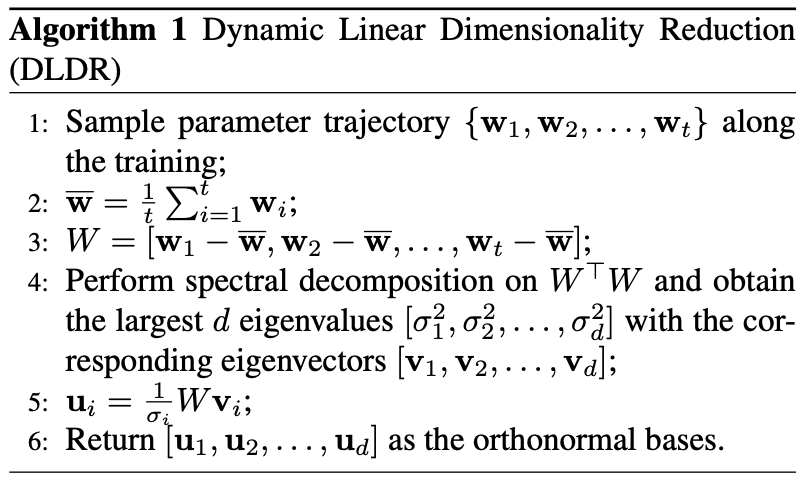
\includegraphics[width=0.9\textwidth]{dldr.png}
\end{figure}
\end{frame}



\begin{frame}
Setting: learning rate 0.1, batch size 128, SGD with momentum of 0.9, 3 trials total \vspace{0,5cm}
\begin{figure}
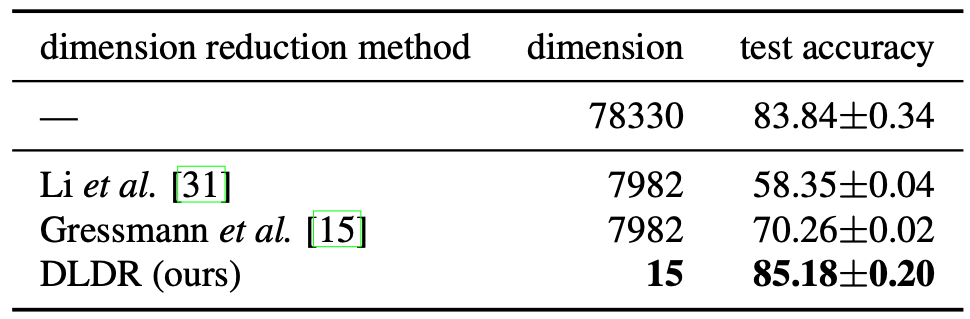
\includegraphics[width=0.99\textwidth]{p-sgd-1}
\end{figure}
\center{Test accuracy of ResNet8 on CIFAR-10} \\
\end{frame}



\begin{frame}
\begin{figure}
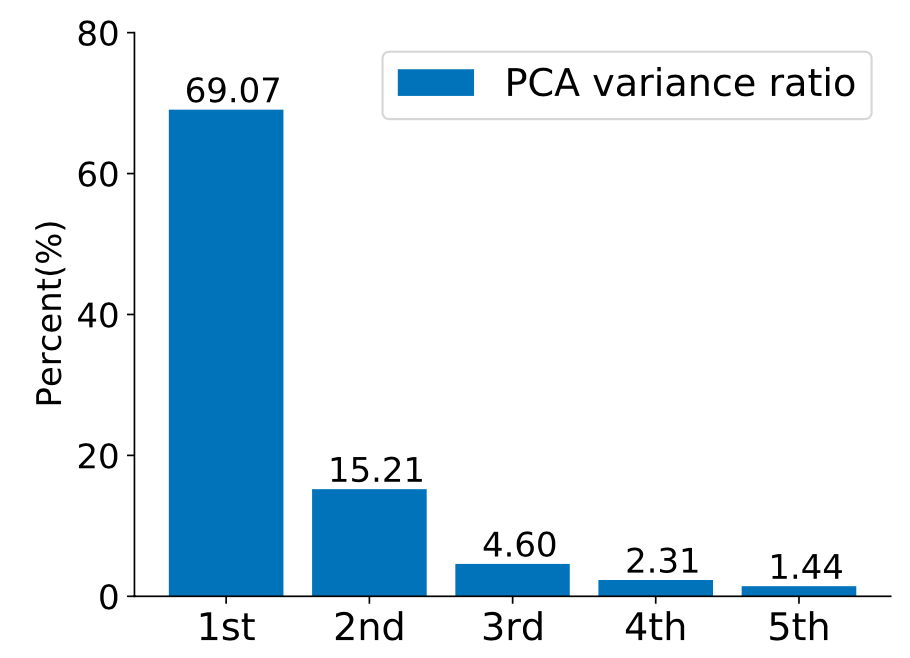
\includegraphics[width=0.6\textwidth]{p-sgd-2}
\end{figure}
\center{PCA ratio of the first 30 epochs training trajectory in the principal directions}
\end{frame}



\begin{frame}
\begin{figure}
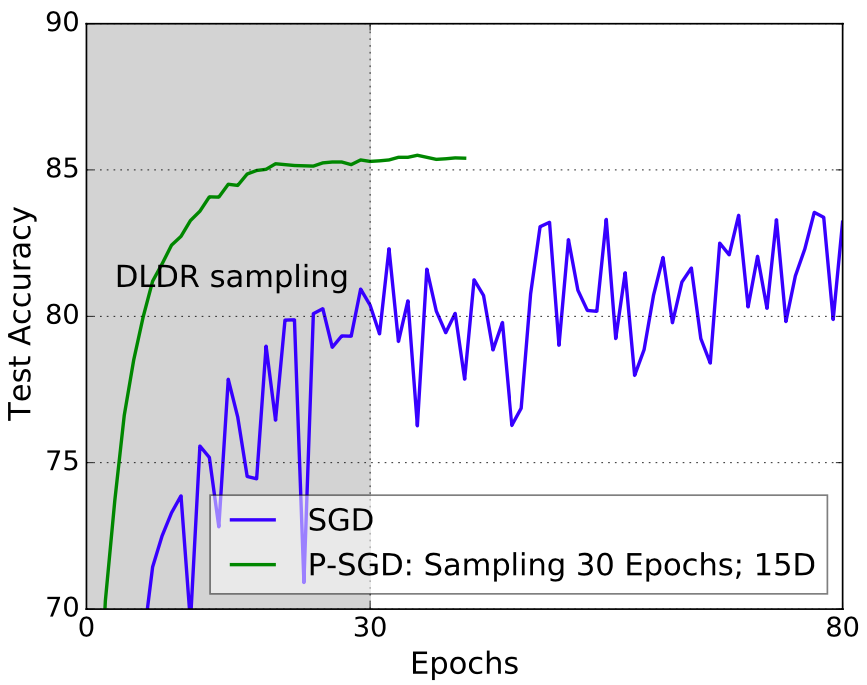
\includegraphics[width=0.6\textwidth]{p-sgd-3}
\center{Training performance of SGD and P-SGD (in 15D subspace)}
\end{figure}
\end{frame}



\section{Agenda}
\begin{frame}
\begin{columns}[c]

\begin{column}{0.5\textwidth}
\begin{center}
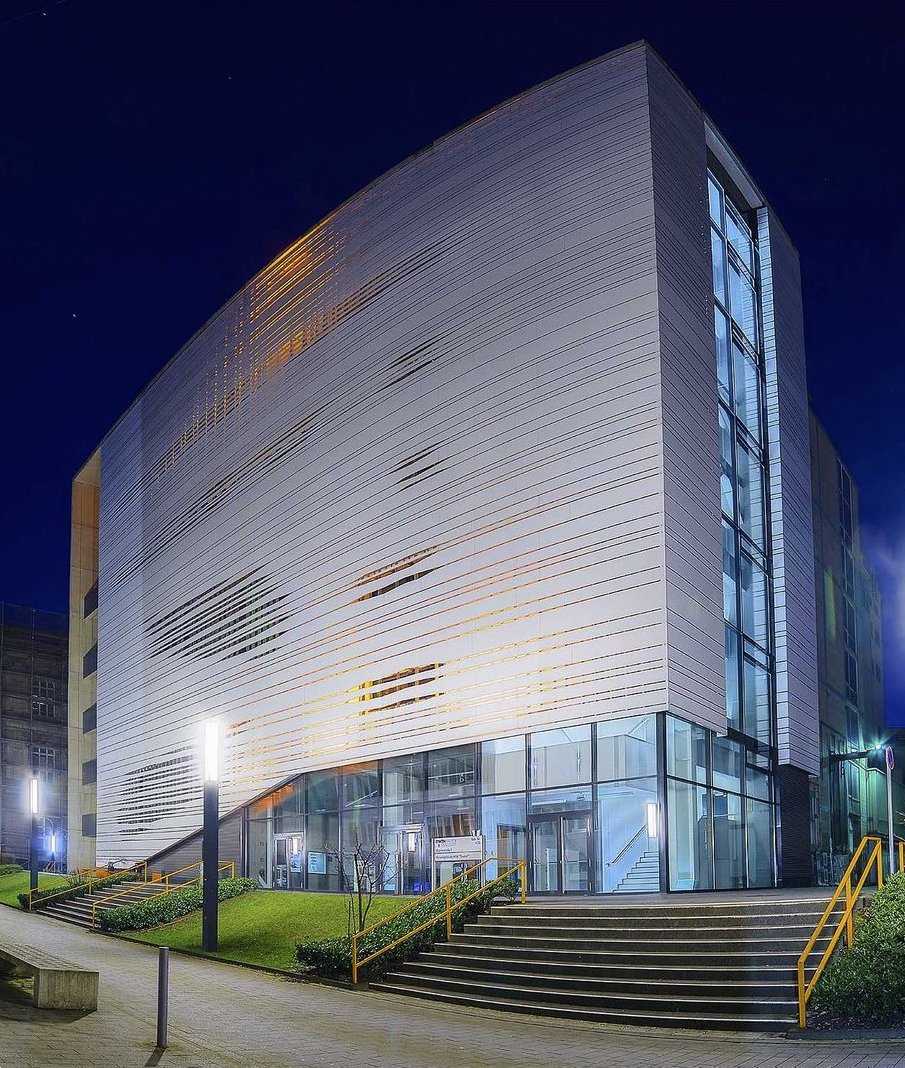
\includegraphics[width=0.9\textwidth]{toaster}
\end{center}
\end{column}

\begin{column}{0.5\textwidth}
\begin{itemize}
\item Dynamic Linear Dimensionality Reduction (DLDR) \vspace{1cm}
\item \textbf{DLDR-based Quasi-Newton Algorithm} \vspace{1cm}
\item Numerical Experiments \vspace{1cm} 
\end{itemize}
\end{column}

\end{columns}
\end{frame}

%%%%%%%%%%%%%%%%%%%%%%%%%%%%%%%%%%%%%%%%%%%%%%%%%%%%%%%%%%%%%%%

\section{DLDR-based Quasi-Newton Algorithm}

\begin{frame}
\begin{itemize}
\item Working in the low-dimensional space has the advantage that we can approximate the Hessian matrix as
\[ H \approx PH_0P^T \]
\item We use the BFGS algorithm with rank two correction update to approximate the inverse Hessian matrix as
\[ \begin{split}
B_{k+1} &= V_k^TB_kV_k + \rho_k\tilde{s}_k\tilde{s}_k^T \\\
y_k &= \tilde{g}_{k+1} - \tilde{g}_k \\\
\rho_k &= (y_k^T\tilde{s}_k)^{-1} \\\
V_k &= I - \rho_ky_k\tilde{s}_k^T
\end{split} \]
where $\tilde{g}_k = P^Tg_k$ is the projected gradient and $\tilde{s}_k = P^T(w_{k+1}-w_k)$ is the projected difference between the parameters
\end{itemize}
\end{frame}



\begin{frame}
\begin{figure}
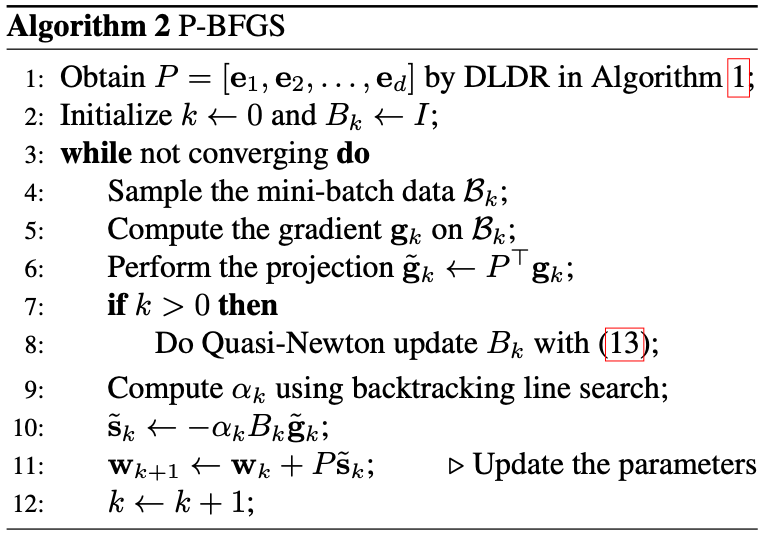
\includegraphics[width=0.8\textwidth]{p-bfgs}
\end{figure}
\end{frame}

%%%%%%%%%%%%%%%%%%%%%%%%%%%%%%%%%%%%%%%%%%%%%%%%%%%%%%%%%%%%%%%

\section{Agenda}
\begin{frame}
\begin{columns}[c]

\begin{column}{0.5\textwidth}
\begin{center}
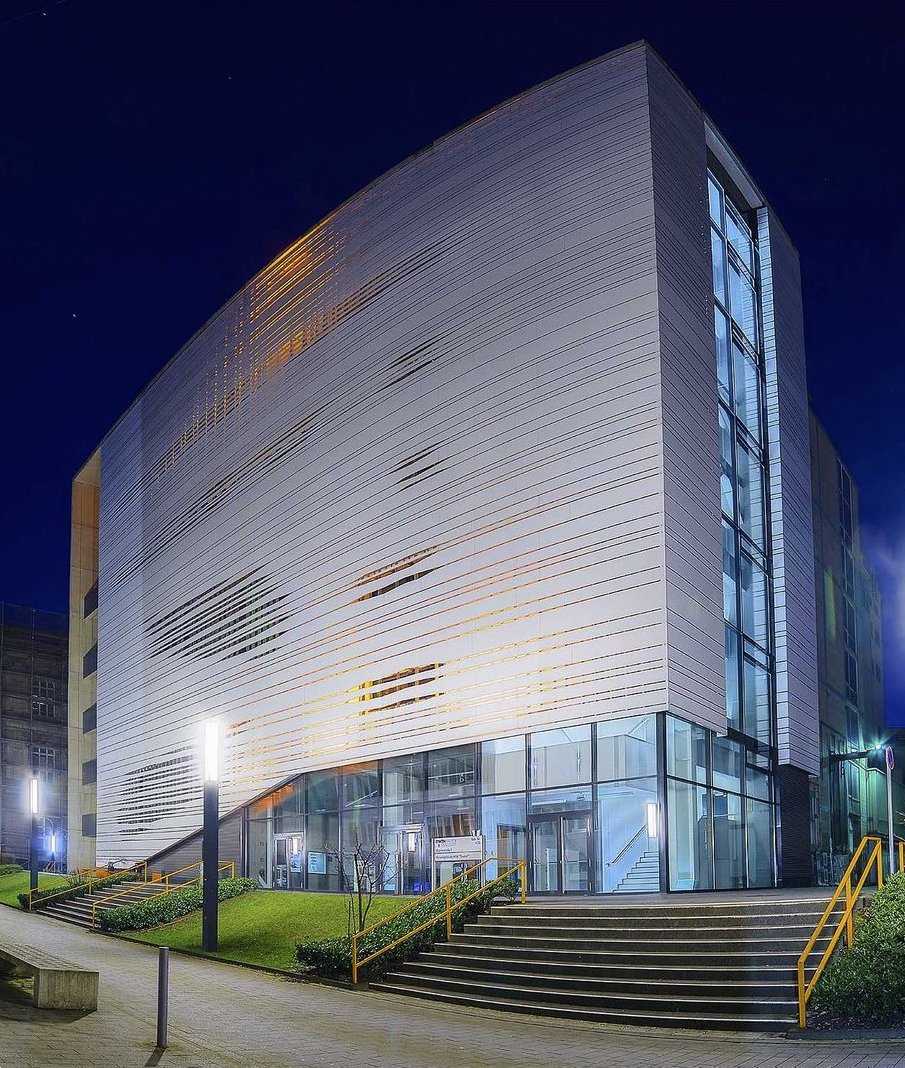
\includegraphics[width=0.9\textwidth]{toaster}
\end{center}
\end{column}

\begin{column}{0.5\textwidth}
\begin{itemize}
\item Dynamic Linear Dimensionality Reduction (DLDR) \vspace{1cm}
\item DLDR-based Quasi-Newton Algorithm \vspace{1cm}
\item \textbf{Numerical Experiments} \vspace{1cm} 
\end{itemize}
\end{column}

\end{columns}
\end{frame}

%%%%%%%%%%%%%%%%%%%%%%%%%%%%%%%%%%%%%%%%%%%%%%%%%%%%%%%%%%%%%%%

\section{Numerical Experiments}

\begin{frame}
\begin{figure}
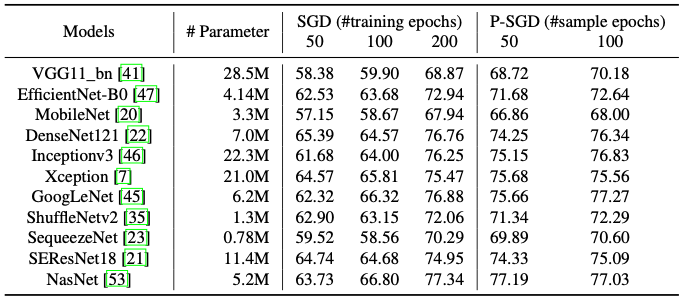
\includegraphics[width=0.99\textwidth]{exp-1}
\end{figure}
\center{Test accuracy on CIFAR-100 for regular training and optimization in 40D subspaces}
\end{frame}



\begin{frame}
\begin{columns}[c]

\begin{column}{0.5\textwidth}
\begin{figure}
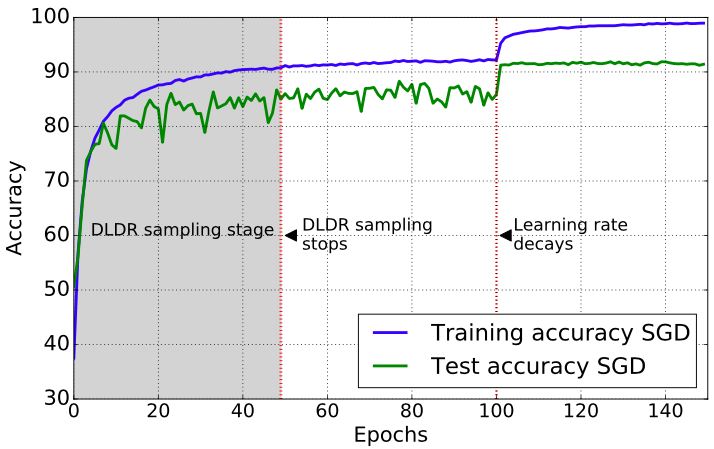
\includegraphics[width=0.99\textwidth]{exp-2}
\end{figure}
\end{column}

\begin{column}{0.5\textwidth}
\begin{figure}
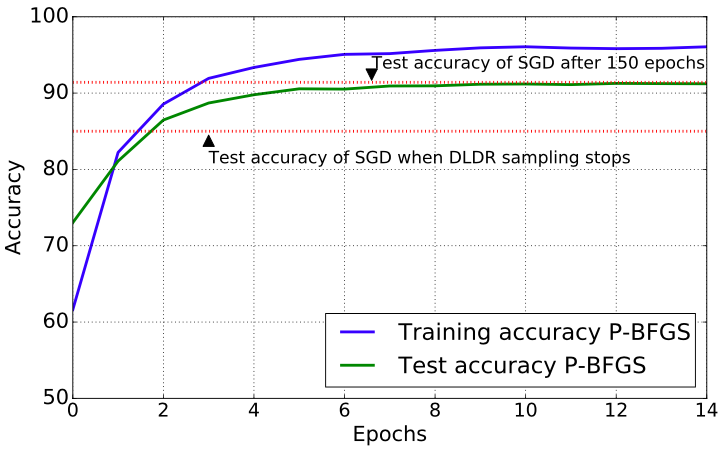
\includegraphics[width=0.99\textwidth]{exp-3}
\end{figure}
\end{column}

\end{columns}
\vspace{1cm}
\center{The accuracy of ResNet20 on CIFAR-10 in different epochs}
\end{frame}



\begin{frame}
\begin{figure}
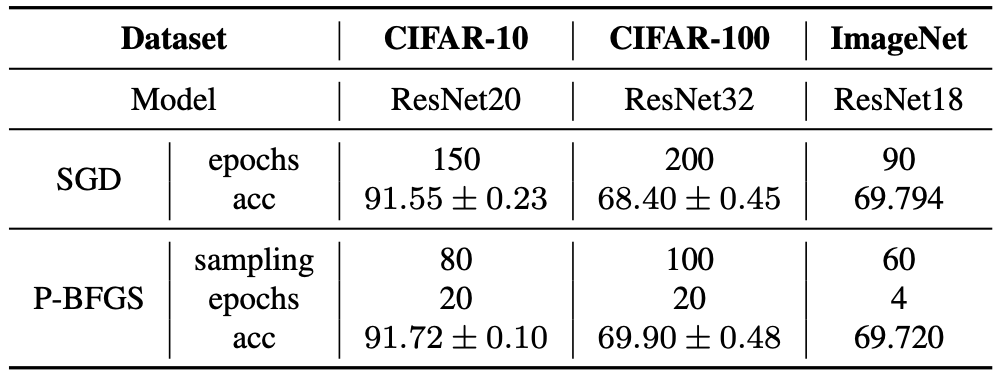
\includegraphics[width=0.99\textwidth]{exp-4}
\end{figure}
\center{Test accuracy obtained by SGD and P-BFGS}
\end{frame}



\begin{frame}
\begin{figure}
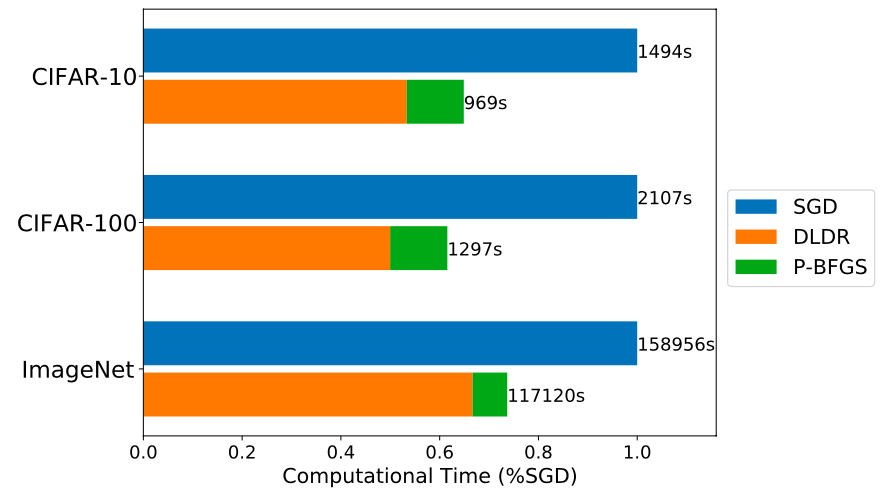
\includegraphics[width=0.85\textwidth]{exp-5}
\end{figure}
\center{Wall-clock time consumption comparisons}
\end{frame}



\begin{frame}
\begin{figure}
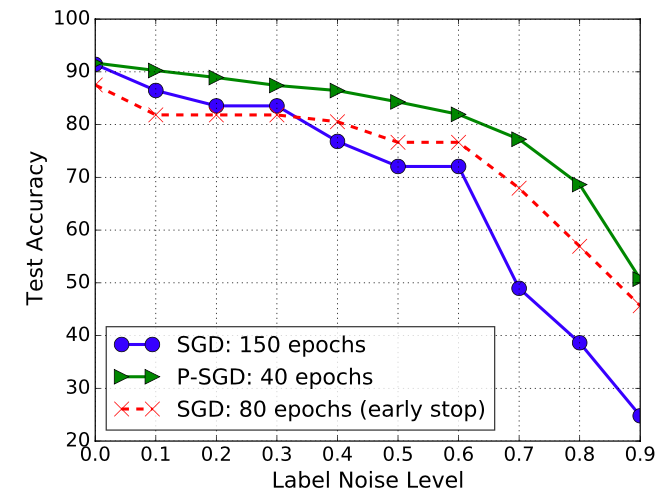
\includegraphics[width=0.65\textwidth]{exp-6}
\end{figure}
\center{The performance under different level of label noise}
\end{frame}

%%%%%%%%%%%%%%%%%%%%%%%%%%%%%%%%%%%%%%%%%%%%%%%%%%%%%%%%%%%%%%%

\section{}

\begin{frame}

\begin{center}

\scalebox{1.5}{\textbf{Are there any questions?}} \\
\ \\


\includegraphics[width=0.95\textwidth]{ask}

\end{center}

\end{frame}

%%%%%%%%%%%%%%%%%%%%%%%%%%%%%%%%%%%%%%%%%%%%%%%%%%%%%%%%%%%%%%%

\section{Ideas for further exploration}

\begin{frame}
\begin{itemize}
\item Test different second order methods
\item Improve the subspace extraction (different sampling strategies, different dimensions, etc.) \vspace{2cm}
\end{itemize}
\center{ \scalebox{1.5}{\textbf{Further ideas?}}} \\
\end{frame}

%%%%%%%%%%%%%%%%%%%%%%%%%%%%%%%%%%%%%%%%%%%%%%%%%%%%%%%%%%%%%%%

\end{document}
